\documentclass{article}
\usepackage[utf8]{inputenc}
\usepackage{graphicx} % Required for inserting images
\graphicspath{ {./images/} }
\usepackage{mathtools} % for math tool slike arrows

\title{Introduction to Quantum Information and Computing Half 2 Lecture 2}
\author{Aayush Acharya, Arnav Negi, Kriti Gupta, Manav Shah, Mohammed Shamil,\\ Shiven Sinha, Shrikara A, Swayam Agrawal, Vineeth Bhat, Yash Adivarekar}
\date{7th February, 2023}

\begin{document}

\maketitle

\section{Classical Logic Gates}

Any boolean function $f:\{0,1\}^n \xrightarrow{} \{0,1\} $ can be written as a propositional formula of $n$ variables.
A universal gate is a gate which can implement any Boolean function $f$ without need to use any other gate type.

\subsection{Reversibility of Logic Gates}

Logical reversibility means that the output can be computed from the input, and vice versa. Reversible functions are bijective. This means that reversible gates (and circuits, i.e. compositions of multiple gates) have the same number of inputs as outputs.

A NOT gate is logically reversible because it can be undone.

The exclusive or XOR gate is irreversible because its two inputs cannot be unambiguously reconstructed from its single output, or alternatively, because information erasure is not reversible. 

A motivation for implementing reversible computing is that they offer to improve the computational energy efficiency of computers.

\section{Shannon Entropy}

Shannon entropy is a measure of the amount of uncertainty or information contained in a quantum state. It is defined as:
$\ \sum_{i} -p_i \log(p_i)$

Example:
Consider a qubit with initial probability distrubution $P:\{0.5,0.5\}$.We reset this qubit and we are asked to calculate the change in entropy.

The initial entropy = $\ -0.5*log(0.5) - 0.5*log(0.5)$\ = $\log(2)$\.

The final entropy is 0 as the qubit is reset and thus no probabilistic measure.

Hence $\Delta S = -log(2)$

\section{Landauer's Principle}

Landauer's principle is a fundamental principle in quantum information theory that relates the amount of irreversible information loss in a computation to the physical process of erasing information. In essence, the principle states that erasing information must necessarily generate entropy, and that the minimum amount of energy required to perform an erasure is proportional to the entropy generated.

It can be formally stated as : Any irreversible operation that erases one bit of information must necessarily generate at least $k_B ln 2$ units of entropy, where $k_B$ is the Boltzmann constant. This means that the minimum energy required to perform an erasure is given by:

$E = k_B T \ln 2$ where $T$ is the temperature of the system in which the erasure is performed.

\section{Clausius Inequality}

The Clausius inequality is a fundamental principle of thermodynamics that places a limit on the amount of work that can be extracted from a system during a thermodynamic process.Mathematically: \\\\
$\Delta Q \geq k_B T \Delta S$ \\\\
Here $\Delta S$ is the decrease in entropy of the system or increase in entropy of environment. $\Delta Q$ denotes the heat lost by the system to the environment.

\section{Demonstrating the relationship between Measurement, Information and Thermodynamics}

The Szilard Engine and Maxwell's Demon are two thought experiments in quantum mechanics that highlight the role of information and measurement in thermodynamics.
\subsection{Szilard Engine}
The Szilard Engine consists of a single particle confined in a box with a partition in the middle. The box is initially in a state of thermal equilibrium with its environment. The partition is moved to one side of the box, and the position of the particle is measured. If the particle is found on one side of the box, then the partition is locked into place, creating a smaller box on that side. This process can be repeated until the particle is confined to a small box, and the work that can be extracted from the process can be used to do useful work. \\\\\
This engine thus demonstrates that measurement and information are intimately connected to thermodynamics. In particular, the act of measuring the position of the particle changes the state of the system, and this change can be used to extract work from the system. This suggests that information is a form of physical resource that can be converted into work.

\section{Reversible Logic Gates}

\subsection{Fredkin Gate} 
Also know as Controlled SWAP Gate

The Fredkin gate has three input bits and three output bits, which we refer to
as a, b, c and a', b', c', respectively. The bit c is a control bit, whose value is not changed by the action of the Fredkin gate, that is, c' = c. The reason c is called the control bit is because it controls what happens to the other two bits, a and b. If c is set to 0 then a and b are left alone, a' = a, b' = b. If c is set to 1, a and b are swapped, a' = b, b' = a. It is easy to see that the Fredkin gate is reversible, because given the output a', b, c', we can determine the inputs a, b, c. In fact, to recover the original inputs a, b and c we need only apply another Fredkin gate to a', b', c

\begin{figure}[htp]
    \centering
    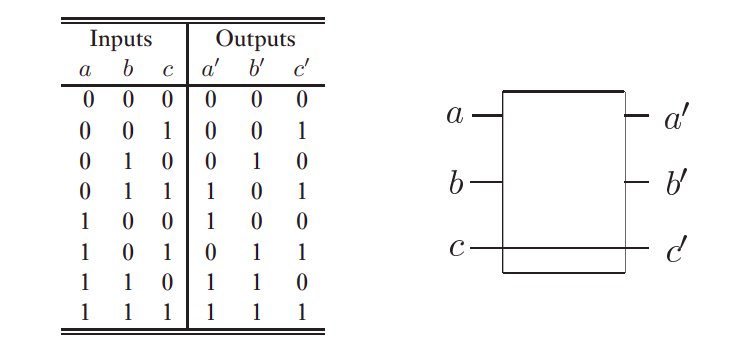
\includegraphics[width=10cm]{fredkin.png}
\end{figure}

The Fredkin gate is not only reversible, it’s a universal logic gate
as well.\\

Reversible AND Gate (R-AND):
\begin{figure}[htp]
    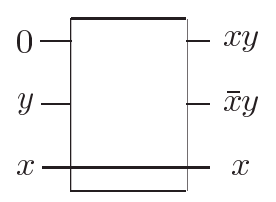
\includegraphics[width=5cm]{rand.png}
\end{figure}
\\

Reversible OR Gate (R-OR):
\begin{figure}[htp]
    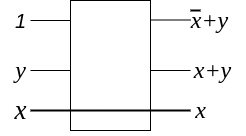
\includegraphics[width=5cm]{ror.png}
\end{figure}
\\

Reversible NOT Gate (R-NOT):
\begin{figure}[htp]
    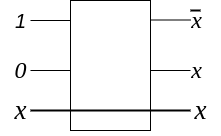
\includegraphics[width=5cm]{rnot.png}
\end{figure}

\subsection{CNOT Gate}
Controlled-NOT Gate: This gate has two input qubits, known as the control qubit and the target qubit.The action of the gate may be described as follows. If the control qubit is set to 0, then the target qubit is left alone. If the control qubit is set to 1, then the target qubit is flipped. The following image shows the circuit and the unitary matrix corresponding to the gate.

\begin{figure}[htp]
    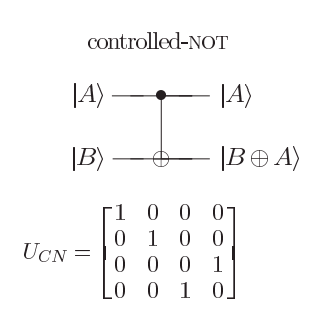
\includegraphics[width=5cm]{cnot.png}
\end{figure}

The reason the CNOT gate is not universal on its own is because it can only generate entangled states where the control and target qubits are either both 0 or both 1. This limits the set of transformations that can be generated.Reversibility is implied from the truth table.
\end{document}
